Looking at the rough outline of the observed period revealed that almost half of the wallets take part in one transaction during that time frame. Roughly 16 percent of the wallets appear two or three times respectively.

\begin{figure}[h]
\centering
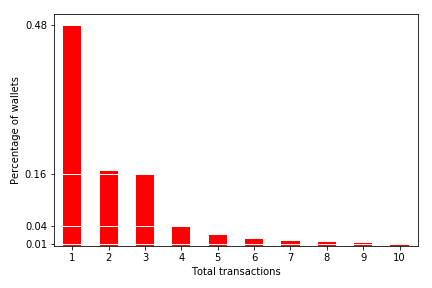
\includegraphics[scale=0.5]{../pics/distribution.png}
\caption{Distribution of total number of transactions}
\end{figure}

\begin{figure*}
\centering
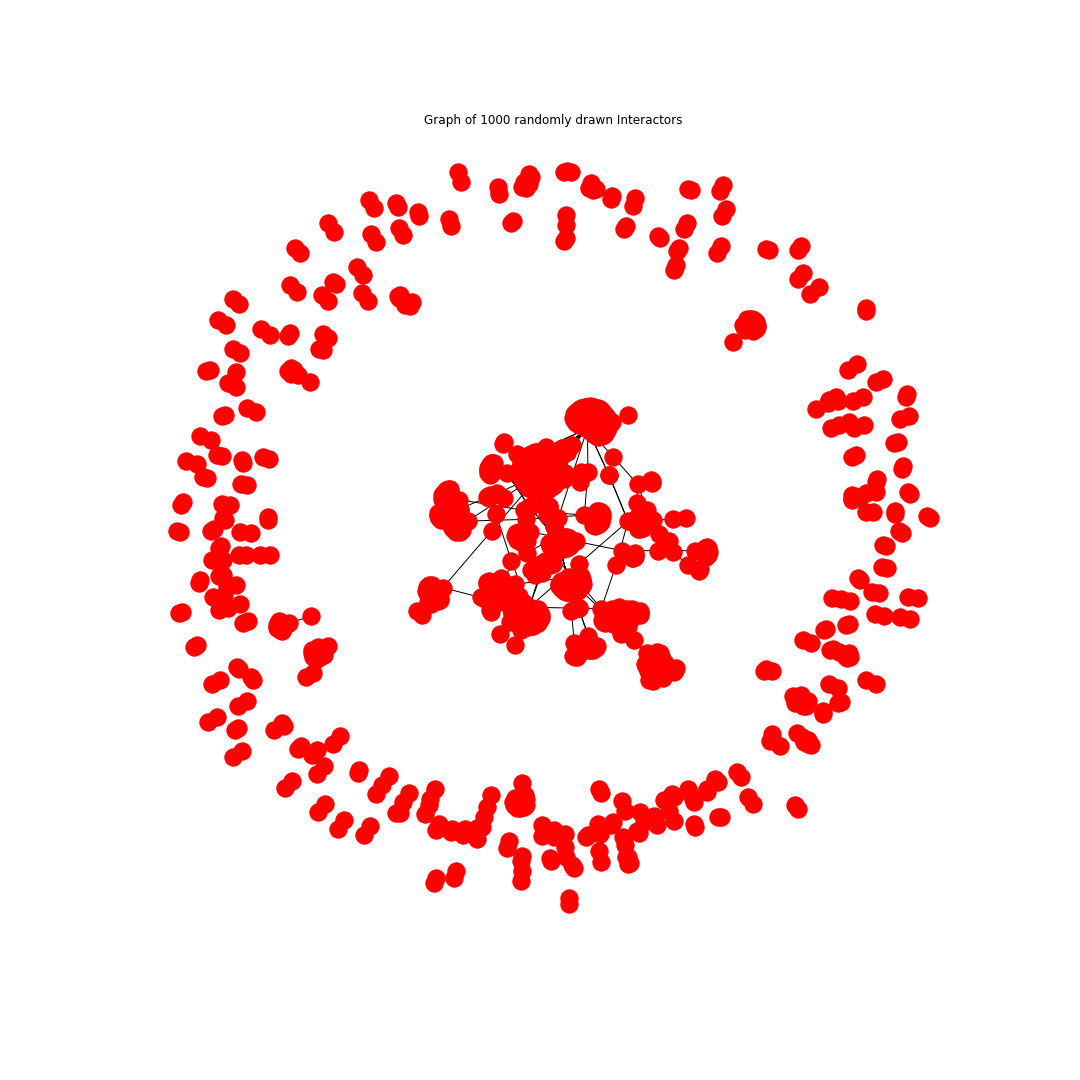
\includegraphics[scale=0.45]{../analysis/graph-subsample-1000.png}
\caption{Graph formed by a subsample of 1000 randomly drawn wallets}
\end{figure*}


\begin{figure*}
\centering
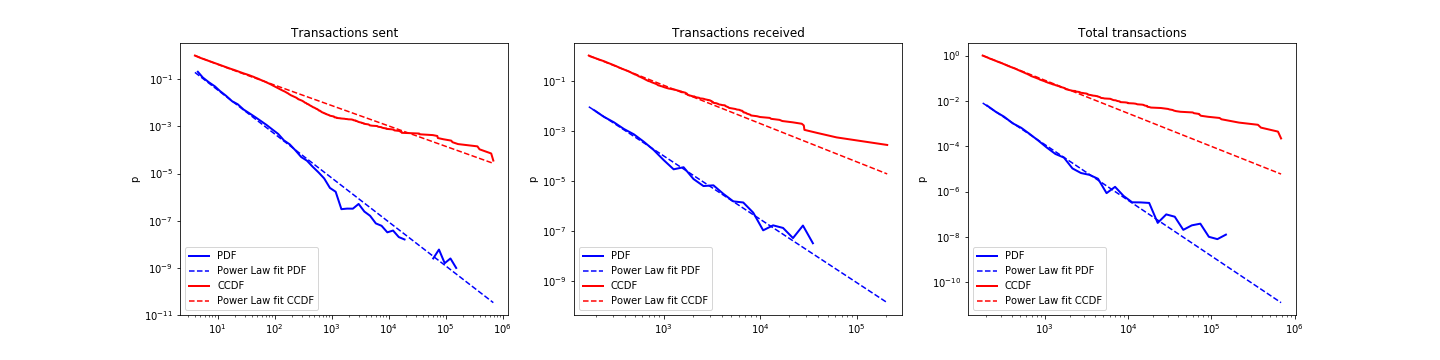
\includegraphics[width=\textwidth]{../analysis/power-law-fit.png}
\caption{Comparison with random graphs}
\end{figure*}
